\setlength{\columnsep}{3pt}
\begin{flushleft}
	
	Let's see some commands to create, update \& delete users in Linux OS.
	
	\paragraph{How to create a new user?}
	\bigskip
	\textbf{useradd}: Create a new user.
	\begin{tcolorbox}[breakable,notitle,boxrule=1pt,colback=pink,colframe=pink]
		\color{black}
		\fontdimen2\font=1em
		Syntax:  useradd username
		\fontdimen2\font=4pt
	\end{tcolorbox}
	On adding a new user, a user have below things set:
	\begin{itemize}
		\item Home directory: \textbf{/home/username}
		\item Default shell: \textbf{/bin/bash}
		\item Primary group: Named same as \textbf{username}
		\item Password: \textbf{No password is set}
	\end{itemize}
	
	\begin{tcolorbox}[breakable,notitle,boxrule=1pt,colback=yellow,colframe=yellow]
		\color{black}
		Note: Some defaults, such as the UID numbers and default password aging rules, are read from the \textbf{/etc/login.defs} file.
	\end{tcolorbox}
	
	Options with \textbf{useradd} command:
	\begin{enumerate}[label=(\alph*)]
		\item \textbf{–g}: Assign primary group.
		\bigskip
		\begin{tcolorbox}[breakable,notitle,boxrule=0pt,colback=pink,colframe=pink]
			\color{black}
			\fontdimen2\font=1em
			Syntax: useradd -g primary\_group\_name username
			\fontdimen2\font=4pt
		\end{tcolorbox}
		Eg:
		\bigskip
		\begin{tcolorbox}[breakable,notitle,boxrule=-0pt,colback=black,colframe=black]
			\color{green}
			\fontdimen2\font=1em
			\# useradd –g javadevl shekhar
			\fontdimen2\font=4pt
		\end{tcolorbox}
		
		\item \textbf{–G}: Assign secondary groups.
		\bigskip
		\begin{tcolorbox}[breakable,notitle,boxrule=0pt,colback=pink,colframe=pink]
			\color{black}
			\fontdimen2\font=1em
			Syntax: useradd -G secondary\_group\_name username
			\fontdimen2\font=4pt
		\end{tcolorbox}
		Eg:
		\bigskip
		\begin{tcolorbox}[breakable,notitle,boxrule=-0pt,colback=black,colframe=black]
			\color{green}
			\fontdimen2\font=1em
			\# useradd –G cdevl,perldevl shekhar
			\fontdimen2\font=4pt
		\end{tcolorbox}
		
		\newpage
		\item \textbf{–u}: Assign specific UID. UID should be more than 500 for normal users.
		\bigskip
		\begin{tcolorbox}[breakable,notitle,boxrule=0pt,colback=pink,colframe=pink]
			\color{black}
			\fontdimen2\font=1em
			Syntax: useradd –u UID username
			\fontdimen2\font=4pt
		\end{tcolorbox}
		Eg:
		\bigskip
		\begin{tcolorbox}[breakable,notitle,boxrule=-0pt,colback=black,colframe=black]
			\color{green}
			\fontdimen2\font=1em
			\# useradd –u 601 shekhar
			\fontdimen2\font=4pt
		\end{tcolorbox}
		
		
		\item \textbf{–s}: Change user shell.
		\bigskip
		\begin{tcolorbox}[breakable,notitle,boxrule=0pt,colback=pink,colframe=pink]
			\color{black}
			\fontdimen2\font=1em
			Syntax: useradd –s shell\_name username
			\fontdimen2\font=4pt
		\end{tcolorbox}
		Eg:
		\bigskip
		\begin{tcolorbox}[breakable,notitle,boxrule=-0pt,colback=black,colframe=black]
			\color{green}
			\fontdimen2\font=1em
			\# useradd –s /sbin/nologin shekhar
			\fontdimen2\font=4pt
		\end{tcolorbox}
		\bigskip
		\begin{tcolorbox}[breakable,notitle,boxrule=-0pt,colback=yellow,colframe=yellow]
			\color{black}
			Note: Shell \textbf{/sbin/nologin} will not allow username to login. Usually used for system users like ftp, squid etc.
		\end{tcolorbox}
		
		
		\item \textbf{–d}: Change user's home directory.
		\bigskip
		\begin{tcolorbox}[breakable,notitle,boxrule=0pt,colback=pink,colframe=pink]
			\color{black}
			\fontdimen2\font=1em
			Syntax: useradd –d directory\_name username
			\fontdimen2\font=4pt
		\end{tcolorbox}
		Eg:
		\bigskip
		\begin{tcolorbox}[breakable,notitle,boxrule=-0pt,colback=black,colframe=black]
			\color{green}
			\fontdimen2\font=1em
			\# useradd –d /mnt/shekar shekhar 
			\fontdimen2\font=4pt
		\end{tcolorbox}
	\end{enumerate}
	
	\bigskip
	\bigskip
	
	\newpage
	
	\paragraph{How to assign or change user’s password?}
	
	\bigskip
	\textbf{passwd}: Assign/change user's password.
	
	\begin{tcolorbox}[breakable,notitle,boxrule=0pt,colback=pink,colframe=pink]
		\color{black}
		\fontdimen2\font=1em
		Syntax: passwd username
		\fontdimen2\font=4pt
	\end{tcolorbox}
	On executing the command, you will be asked to set password twice.
	
	\begin{tcolorbox}[breakable,notitle,boxrule=0pt,colback=yellow,colframe=yellow]
		\color{black}
		Note: 
		\begin{itemize}
			\item Root user or superuser can set the password of any user.
			\item Local user can set their own password, but not of anyone else.
		\end{itemize}

	\end{tcolorbox}
	
	Options with \textbf{passwd} command:
	
	\begin{itemize}
		\item \textbf{- -stdin}: Change password by providing it on command line itself.
		\begin{tcolorbox}[breakable,notitle,boxrule=0pt,colback=pink,colframe=pink]
			\color{black}
			\fontdimen2\font=1em
			Syntax: echo “new\_password” | passwd ---stdin username
			\fontdimen2\font=4pt
		\end{tcolorbox}
		Eg:
		\bigskip
		\begin{tcolorbox}[breakable,notitle,boxrule=-0pt,colback=black,colframe=black]
			\color{green}
			\fontdimen2\font=1em
			\# echo “shekhar@12345” | passwd ---stdin shekhar
			\fontdimen2\font=4pt
		\end{tcolorbox}
	\end{itemize}
\newpage

\newpage
\paragraph{How to change user’s password attributes?}

\bigskip
\textbf{chage}: Changing the password aging information for user.

\begin{tcolorbox}[breakable,notitle,boxrule=0pt,colback=pink,colframe=pink]
	\color{black}
	\fontdimen2\font=1em
	Syntax: chage username
	\fontdimen2\font=4pt
\end{tcolorbox}
Eg:
\begin{figure}[h!]
	\centering
	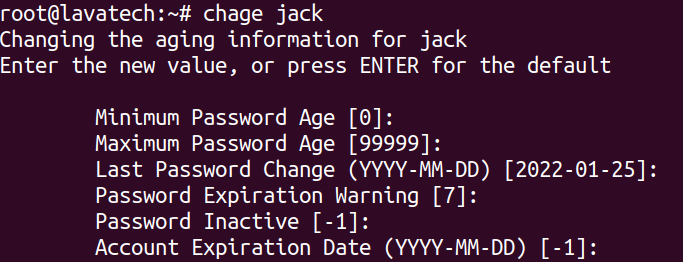
\includegraphics[scale=.5]{content/chapter4/images/chage1.png}
	\caption{Sample output}
	\label{fig:command_prompt5}
\end{figure}

Options with \textbf{chage} command:

\begin{itemize}
	\item \textbf{-l}: Show account aging information.
	\begin{tcolorbox}[breakable,notitle,boxrule=0pt,colback=pink,colframe=pink]
		\color{black}
		\fontdimen2\font=1em
		Syntax: chage -l username
		\fontdimen2\font=4pt
	\end{tcolorbox}
	Eg:
	\bigskip
	\begin{figure}[h!]
		\centering
		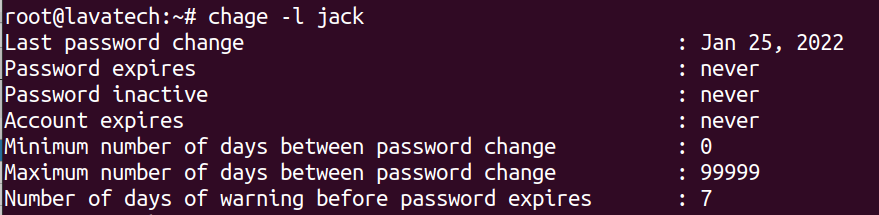
\includegraphics[scale=.5]{content/chapter4/images/chage2.png}
		\caption{Sample output}
		\label{fig:command_prompt8}
	\end{figure}
\end{itemize}

\newpage

\paragraph{Switch between users}
\begin{itemize}
	\item \textbf{su}: Allows a user to switch to a different user account. If a username is not specified, the root account is implied.
		\begin{tcolorbox}[breakable,notitle,boxrule=0pt,colback=pink,colframe=pink]
		\color{black}
		\fontdimen2\font=1em
		Syntax: su [-] [username]
		\fontdimen2\font=4pt
	\end{tcolorbox}
	Eg:
	\bigskip
	\begin{tcolorbox}[breakable,notitle,boxrule=-0pt,colback=black,colframe=black]
		\color{green}
		\fontdimen2\font=1em
		\# su - jack
		\fontdimen2\font=4pt
	\end{tcolorbox}
	What is used of "-" in su command?
	\begin{itemize}
		\item The command \textbf{"su username"} starts a non-login shell, while the command \textbf{"su - username"} starts a login shell. 
		\item The main distinction is \textbf{"su -"} sets up the shell environment as if this were a clean login as that user, while \textbf{"su"} just starts a shell as that user with the current environment settings.
	\end{itemize}
\end{itemize}

\paragraph{Running command as root with sudo}
\begin{itemize}
	\item \textbf{sudo}: Allows a user to be permitted to run a command as root, or as another user,
	based on settings in the /etc/sudoers file.
	\begin{tcolorbox}[breakable,notitle,boxrule=0pt,colback=pink,colframe=pink]
		\color{black}
		\fontdimen2\font=1em
		Syntax: sudo command
		\fontdimen2\font=4pt
	\end{tcolorbox}
	Eg:
	\bigskip
	\begin{tcolorbox}[breakable,notitle,boxrule=-0pt,colback=black,colframe=black]
		\color{green}
		\fontdimen2\font=1em
		\$ sudo useradd raman
		\fontdimen2\font=4pt
	\end{tcolorbox}
\end{itemize}

	
	\newpage
	
	\paragraph{How to modify an existing user?}
	\bigskip
	\textbf{usermod}: Modify existing user.
	\newline
	Options with \textbf{usermod} command:
	\begin{enumerate}[label=(\alph*)]
		\item \textbf{–g}: Change user's primary group.
		\bigskip
		\begin{tcolorbox}[breakable,notitle,boxrule=0pt,colback=pink,colframe=pink]
			\color{black}
			\fontdimen2\font=1em
			Syntax: usermod –g primary\_group username
			\fontdimen2\font=4pt
		\end{tcolorbox}
		Eg:
		\bigskip
		\begin{tcolorbox}[breakable,notitle,boxrule=-0pt,colback=black,colframe=black]
			\color{green}
			\fontdimen2\font=1em
			\# usermod –g cdevl shekhar
			\fontdimen2\font=4pt
		\end{tcolorbox}
		
		\item \textbf{–G}: Change user's secondary group.
		\bigskip
		\begin{tcolorbox}[breakable,notitle,boxrule=0pt,colback=pink,colframe=pink]
			\color{black}
			\fontdimen2\font=1em
			Syntax: usermod -G secondary\_group\_name username
			\fontdimen2\font=4pt
		\end{tcolorbox}
		Eg:
		\bigskip
		\begin{tcolorbox}[breakable,notitle,boxrule=-0pt,colback=black,colframe=black]
			\color{green}
			\fontdimen2\font=1em
			\# usermod –G javadevl shekhar
			\fontdimen2\font=4pt
		\end{tcolorbox}
		
		
		\item \textbf{–L}: Lock (i.e. disable) user.
		\bigskip
		\begin{tcolorbox}[breakable,notitle,boxrule=0pt,colback=pink,colframe=pink]
			\color{black}
			\fontdimen2\font=1em
			Syntax: usermod -L username
			\fontdimen2\font=4pt
		\end{tcolorbox}		
		
		\item \textbf{–U}: Unlock user account.
		\bigskip
		\begin{tcolorbox}[breakable,notitle,boxrule=0pt,colback=pink,colframe=pink]
			\color{black}
			\fontdimen2\font=1em
			Syntax: usermod –U username
			\fontdimen2\font=4pt
		\end{tcolorbox}
		
		\item \textbf{–s}: Change user's login shell.
		\bigskip
		\begin{tcolorbox}[breakable,notitle,boxrule=0pt,colback=pink,colframe=pink]
			\color{black}
			\fontdimen2\font=1em
			Syntax: usermod –s shell\_name username
			\fontdimen2\font=4pt
		\end{tcolorbox}
		Eg:
		\bigskip
		\begin{tcolorbox}[breakable,notitle,boxrule=-0pt,colback=black,colframe=black]
			\color{green}
			\fontdimen2\font=1em
			\# usermod –s /bin/ksh shekhar
			\fontdimen2\font=4pt
		\end{tcolorbox}
		
		\newpage
		\item \textbf{–d}: Change user's home directory.
		\item \textbf{-m}: Create user's new home directory.
		\bigskip
		\begin{tcolorbox}[breakable,notitle,boxrule=0pt,colback=pink,colframe=pink]
			\color{black}
			\fontdimen2\font=1em
			Syntax: usermod –d directory\_name username -m
			\fontdimen2\font=4pt
		\end{tcolorbox}
		Eg:
		\bigskip
		\begin{tcolorbox}[breakable,notitle,boxrule=-0pt,colback=black,colframe=black]
			\color{green}
			\fontdimen2\font=1em
			\# usermod –d /opt/java shekhar -m
			\fontdimen2\font=4pt
		\end{tcolorbox}
	\end{enumerate}
	
	\bigskip
	\bigskip
	
	\newpage
	
	\paragraph{How to delete a user?}
	
	\bigskip
	\begin{tcolorbox}[breakable,notitle,boxrule=-0pt,colback=red,colframe=red]
		\color{white}
		Standard Practice: You should not delete a user if they leave	 the organization. You
		should lock their account.
	\end{tcolorbox}
	
	
	
	\textbf{userdel}: Delete user \& remove it's entry from \textbf{/etc/passwd} and \textbf{/etc/shadow} files.
	\begin{tcolorbox}[breakable,notitle,boxrule=0pt,colback=pink,colframe=pink]
		\color{black}
		\fontdimen2\font=1em
		Syntax: userdel username
		\fontdimen2\font=4pt
	\end{tcolorbox}
	Eg:
	\begin{tcolorbox}[breakable,notitle,boxrule=-0pt,colback=black,colframe=black]
		\color{green}
		\fontdimen2\font=1em
		\# userdel shekhar
		\fontdimen2\font=4pt
	\end{tcolorbox}

	\begin{tcolorbox}[breakable,notitle,boxrule=-0pt,colback=yellow,colframe=yellow]
		\color{black}
		Note: userdel command does not delete user's home directory by default.
	\end{tcolorbox}	

	Options with \textbf{userdel} command:
	\begin{itemize}
		\item \textbf{-r}: Delete user along with home directory.
		\begin{tcolorbox}[breakable,notitle,boxrule=0pt,colback=pink,colframe=pink]
			\color{black}
			\fontdimen2\font=1em
			Syntax: userdel -r username
			\fontdimen2\font=4pt
		\end{tcolorbox}
		Eg:
		\begin{tcolorbox}[breakable,notitle,boxrule=-0pt,colback=black,colframe=black]
			\color{green}
			\fontdimen2\font=1em
			\# userdel -r shekhar
			\fontdimen2\font=4pt
		\end{tcolorbox}
	\end{itemize}
	
\end{flushleft}

\newpage

